\documentclass{article}
\usepackage[margin=2.5cm, top=4cm, headheight=25pt]{geometry}
\usepackage{amsmath, amssymb, enumitem, fancyhdr, graphicx}
\usepackage[indent=20pt]{parskip}
\usepackage[hidelinks]{hyperref}
\usepackage{xcolor}
\usepackage{listings}
\usepackage{subcaption}
\usepackage{url}
\usepackage[most]{tcolorbox}
\usepackage{lastpage}

\tcbuselibrary{listingsutf8} % Support for lstlistings within tcolorbox

\newtcolorbox[auto counter, number within=section]{question}[1][]{%
    colframe=gray!80,                      % Dark gray frame
    colback=gray!5,                       % Light gray background
    coltitle=black,                        % Black title
    title=\textbf{Question~\thetcbcounter}, % Bold title
    fonttitle=\bfseries\large,             % Subtle title font size
    rounded corners,                   % Slightly more rounded corners
    boxrule=0.25mm,                         % Thinner border for a sleek look
    enhanced,                              % Enhanced box features
    attach boxed title to top left={xshift=2mm, yshift=-2mm},
    boxed title style={colframe=gray!80, colback=gray!5, boxrule=0.25mm},
    % Title styling
    #1
}

\bibliographystyle{IEEEtran}
\graphicspath{{./images/}}

% -- Custom Variables --
\def\me{Rajdeep Gill 7934493}
\def\course{ECE 4260}
\def\labsection{A01}

\def\labno{2}
\def\title{Assignment 2}

% -- Styling for code snippets --
\lstset{
    basicstyle=\ttfamily\scriptsize,           % Basic font style
    keywordstyle=\color{blue},            % Keywords color
    commentstyle=\color{gray},            % Comments color
    stringstyle=\color{teal},             % Strings color
    numbers=left,                         % Line numbers on the left
    numberstyle=\tiny\color{gray},        % Line number style
    stepnumber=1,                         % Line number step
    numbersep=10pt,                       % Space between line numbers and code
    backgroundcolor=\color{lightgray!10}, % Background color
    frame=single,                         % Adds a frame around the code
    breaklines=true,                      % Line breaking for long lines
    captionpos=b,                         % Caption position
    showspaces=false,                     % Don't show spaces
    showstringspaces=false                % Don't show spaces in strings
}
\renewcommand{\lstlistingname}{Code Snippet}

\renewcommand{\arraystretch}{1.2} % For less-ugly tables
\setlength\parindent{0pt}

%----- Samples 
% Questions:
%   \begin{question}[title=Custom Question Title]
%       Question details
%   \end{question}

% Tables:
%   \begin{table}[htbp]
%       \centering
%       \caption{Table Caption}
%       \begin{tabular}{ll}
%           \toprule
%           \textbf{Column 1} & \textbf{Column 2} \\
%           \midrule
%           Row 1 & Row 2 \\
%           Row 3 & Row 4 \\
%           \bottomrule
%       \end{tabular}
%   \end{table} 

% Figures:
%   Single figure:
%       \begin{figure}[htbp]
%           \centering
%           \includegraphics[width=0.5\textwidth]{example-image}
%           \caption{Figure Caption}
%       \end{figure}
%   Multiple figures:
%       \begin{figure}[htbp]
%           \centering
%           \begin{subfigure}[b]{0.5\textwidth}
%               \includegraphics[width=\textwidth]{example-image-a}
%               \caption{First subfigure}
%           \end{subfigure}
%           \begin{subfigure}[b]{0.5\textwidth}
%               \includegraphics[width=\textwidth]{example-image-b}
%               \caption{Second subfigure}
%           \end{subfigure}
%           \caption{Main figure}
%       \end{figure}

\begin{document}

% --------------------------------------------------------------------------------
% TITLE
% --------------------------------------------------------------------------------

\begin{center}
    \huge \title

    \vspace{2mm}
    \hrule

    \vspace{4mm}
    \large \me

    \vspace{2mm}
    \large \course~\labsection

    \vspace{2mm}
    \today
\end{center}

\vspace{4mm}

% --------------------------------------------------------------------------------
% END TITLE
% --------------------------------------------------------------------------------

\newpage


\vspace{1cm}
\newpage

\pagestyle{fancy}
\fancyhead[L]{\large Assignment \labno}
\fancyhead[R]{\large \me}

\fancyfoot[C]{Page \thepage~of~\pageref{LastPage}}

% --------------------------------------------------------------------------------
% BODY
% --------------------------------------------------------------------------------

\section{Problem 1}

Given that it is an LTI system, the responses to the two new inputs can be derived from the given response.

\begin{enumerate}[label=1.\arabic*]
    \item We can express $x_2(t)$ as:
        \begin{align*}
            x_2(t) &= x_1(t) - x(t-2) \\
            \implies y_2(t) &= y_1(t) - y(t-2) \\
            &= 2\Lambda(t-1) - 2\Lambda(t-2)
        \end{align*} 
    \item We can express $x_3(t)$ as:
        \begin{align*}
            x_3(t) &= x(t+1) + x(t) \\
            \implies y_3(t) &= y(t+1) + y(t) \\
            &= 2\Lambda(t) + 2\Lambda(t-1)
        \end{align*}
\end{enumerate}

The plots of the inputs and outputs can be seen in \autoref{fig:p1}.

\begin{figure}[ht!]
    \centering
    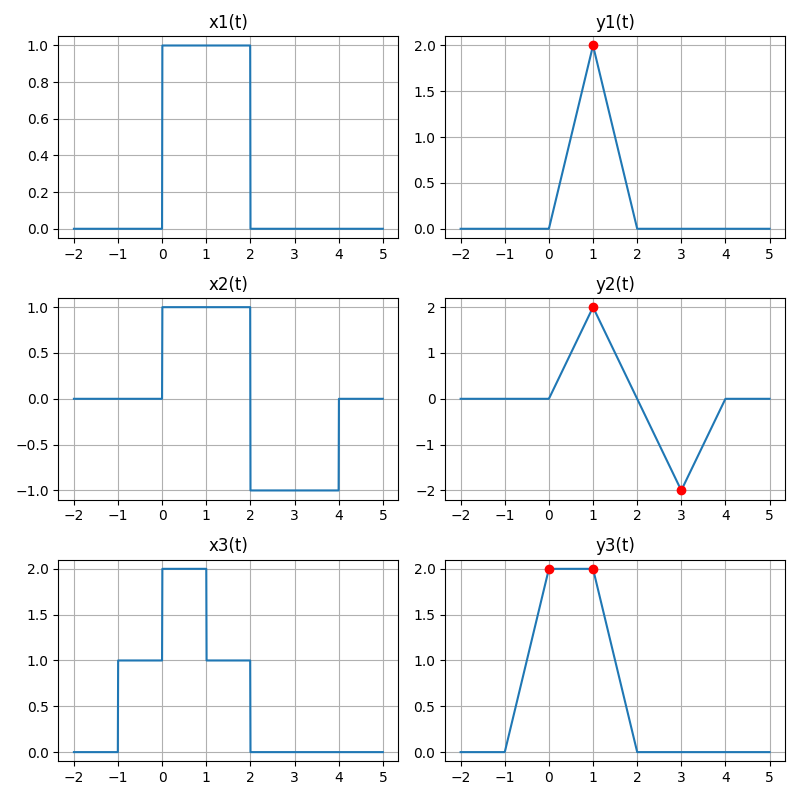
\includegraphics[width=0.75\textwidth]{plot.png}
    \caption{Plots of the inputs and outputs}
    \label{fig:p1}
\end{figure}

\section{Problem 2}
We can express $h(t)$ as a sinc function:
\begin{align*}
    \text{sinc}(t) &= \frac{\sin(\pi t)}{\pi t} \\
    \implies \frac{\sin(4[t-1])}{\pi(t-1)} &= \frac{\sin(\pi \frac{4[t-1]}{\pi})}{\pi(t-1)} \\
    &= \frac{\frac{4}{\pi} \sin(\pi \frac{4[t-1]}{\pi})}{\pi \frac{4}{\pi}(t-1)} \\
    &= \frac{4}{\pi} \text{sinc}\left(\frac{4[t-1]}{\pi}\right)
\end{align*}

In frequency domain, using the tables, we find that the impulse response of a sinc function is a rectangle function. We also apply the time scaling property and time shifting property of the fourier transform:
\begin{align*}
    \text{sinc(t)} &\xrightarrow{\mathcal{F}} \text{rect}(f) \\
    \text{sinc}(a(t-t_0)) &\xrightarrow{\mathcal{F}} \frac{1}{|a|}\text{rect}(f/a) \times e^{-j2\pi f t_0}
\end{align*}

We have that $a = 4/\pi$ and $t_0 = 1$. Thus, the fourier transform of $h(t)$ is:
\begin{align*}
    H(f) &= \text{rect}\left(\frac{\pi f}{4}\right) \times e^{-j2\pi f} \\
\end{align*}


\begin{enumerate}[label=2.\arabic*]
    \item We can rewrite $x_1(t)$ as follows:
    \begin{align*}
        x_1(t) = \frac{\sin(4[t+1])}{\pi(t+1)} = \frac{\frac{4}{\pi}\sin\left(\pi \frac{4[t+1]}{\pi}\right)}{\pi \frac{4}{\pi}(t+1)} = \frac{4}{\pi} \text{sinc}\left(\frac{4[t+1]}{\pi}\right)
    \end{align*}
    Similarly the fourier transform of $x_1(t)$ is:
    \begin{align*}
        X_1(f) = \frac{\pi}{4} \text{rect}\left(\frac{\pi f}{4}\right) \times e^{j2\pi f} \\
    \end{align*}

    The output of the system is given by:
    \begin{align*}
        Y_1(f) &= H(f) \cdot X_1(f) \\
        &= \left(\frac{\pi}{4} \text{rect}\left(\frac{\pi f}{4}\right) \times e^{-j2\pi f}\right) \times \left(\frac{\pi}{4} \text{rect}\left(\frac{\pi f}{4}\right) \times e^{j2\pi f}\right) \\
        &= \frac{\pi}{4} \text{rect}\left(\frac{\pi f}{4}\right)\\
    \end{align*}

    Taking the inverse fourier transform of the rect function, with the time scaling:
    \begin{align*}
        \mathcal{F}^{-1}\left\{\text{rect}\left(\frac{f}{a}\right) \right\} &= |a| \text{sinc}(at) \\
        \text{Where } a &= 4/\pi \\
        \implies \text{rect}\left(\frac{\pi f}{4}\right) &\xrightarrow{\mathcal{F}^{-1}} \frac{4}{\pi} \text{sinc}\left(\frac{4t}{\pi}\right)
    \end{align*}

    Thus, the output of the system is:
    \begin{align*}
        y_1(t) &= \frac{\pi}{4} \times \frac{4}{\pi} \text{sinc}\left(\frac{4t}{\pi}\right) \\
        &= \boxed{\text{sinc}\left(\frac{4t}{\pi}\right)}
    \end{align*}

    \item We can rewrite $x_2(t)$ as follows:   
    \begin{align*}
        x_2(t) &= \left(\frac{\sin(2t)}{\pi t}\right)^2 \\
        &= \left(\frac{\frac{2}{\pi} \sin\left(\pi \frac{2t}{\pi}\right)}{\pi \times \frac{2t}{\pi}}\right)^2 \\
        &= \frac{4}{\pi^2} \text{sinc}^2\left(\frac{2t}{\pi}\right) \\
        &= \frac{4}{\pi^2} \text{sinc}\left(\frac{2t}{\pi}\right) \times \text{sinc}\left(\frac{2t}{\pi}\right)
    \end{align*}

    Since multiplication in the time domain is convolution in the frequency domain, we can find the fourier transform of $x_2(t)$ as follows:
    \begin{align*}
        \text{sinc}\left(\frac{2t}{\pi}\right) &\xrightarrow{\mathcal{F}} \frac{\pi}{2}\text{rect}\left(\frac{\pi f}{2}\right) \\
    \end{align*}

    The convolution of two rectangular functions of the same width is a triangle function. Thus, the fourier transform of $x_2(t)$ is:
    \begin{align*}
        X_2(f) &= \frac{4}{\pi^2}\left(
            \frac{\pi}{2}\text{rect}\left(\frac{\pi f}{2}\right) \ast \frac{\pi}{2}\text{rect}\left(\frac{\pi f}{2}\right)
        \right) \\
        &= \text{rect}\left(\frac{\pi f}{2}\right) \ast \text{rect}\left(\frac{\pi f}{2}\right) \\
    \end{align*}

    The output in the frequency domain is:
    \begin{align*}
        Y_2(f) &= H(f) \cdot X_2(f) \\
        &= \frac{\pi}{4}\left( \text{rect}\left(\frac{\pi f}{4}\right) \times e^{-j2\pi f}\right) \times \left(\text{rect}\left(\frac{\pi f}{2}\right) \ast \text{rect}\left(\frac{\pi f}{2}\right)\right) \\
    \end{align*}

    Since the rectangle function is $1$ for $|f| \leq 1/2$, mutliplying by the rectangular function on the outside is essentially mutliplying by 1. Thus, the output in the frequency domain is:
    \begin{align*}
        Y_2(f) &=  \left(\frac{\pi}{4}\text{rect}\left(\frac{\pi f}{2}\right) \ast \text{rect}\left(\frac{\pi f}{2}\right)\right) \times e^{-j2\pi f} \\
    \end{align*}

    The convolution in the frequency domain is equivalent to multiplication in the time domain. Thus, the output in the time domain is:
    \begin{align*}
        \mathcal{F}^{-1}\left(\frac{\pi}{4}\text{rect}\left(\frac{\pi f}{2}\right) \ast \text{rect}\left(\frac{\pi f}{2}\right)\right) &= \frac{\pi}{4} \mathcal{F}^{-1}\left(\text{rect}\left(\frac{\pi f}{2}\right)\right) \times \mathcal{F}^{-1}\left(\text{rect}\left(\frac{\pi f}{2}\right)\right) \\
        &= \frac{\pi}{4} \left(\frac{2}{\pi} \text{sinc}\left(\frac{2t}{\pi}\right)\right) \times \left(\frac{2}{\pi} \text{sinc}\left(\frac{2t}{\pi}\right)\right) \\
        &= \frac{1}{\pi}\left(\text{sinc}\left(\frac{2t}{\pi}\right)\right)^2 \
    \end{align*}

    The multiplication by the exponential term in the frequency domain is equivalent to a time shift, $t_0 = 1$,  in the time domain. Thus, the output in the time domain is:
    \begin{align*}
        y_2(t) = \boxed{\frac{1}{\pi}\left(\text{sinc}\left(\frac{2(t-1)}{\pi}\right)\right)^2}
    \end{align*}

\end{enumerate}

\section{Problem 3}
\begin{enumerate}[label=3.\arabic*]
    \item We can find the fourier series coefficients as follows:
    \begin{align*}
        g_n &= \frac{1}{T} \int_{0}^{T} g(t) e^{-j2\pi n t/T} dt \\
        &= \frac{1}{2} \int_{0}^{2} t^2e^{-j\pi n t} dt \\
    \end{align*}
    We can solve this integral by doing integration by parts twice:
    \begin{align*}
        \int t^2 e^{at} dt = \frac{t^2 e^{at}}{a} - \frac{2t e^{at}}{a^2} - \frac{2 e^{at}}{a^3}
    \end{align*}

    We have that $a = -j\pi n$:
    \begin{align*}
        2g_n &= \left\{\frac{t^2 e^{-j\pi n t}}{-j\pi n} - \frac{2t e^{-j\pi n t}}{(-j\pi n)^2} - \frac{2 e^{-j\pi n t}}{(-j\pi n)^3}\right\} \Bigg|_{0}^{2} \\
        &= \left(\frac{4 e^{-2j\pi n}}{-j \pi n} - \frac{4 e^{-2j\pi n}}{(-j\pi n)^2} - \frac{2 e^{-2j\pi n}}{(-j\pi n)^3}\right) - \left(-\frac{2}{(-j\pi n )^3}\right) \\
        g_n &= \frac{2e^{-2j\pi n}}{-j \pi n} - \frac{2e^{-2j\pi n}}{(-j\pi n)^2} - \frac{e^{-2j\pi n}}{(-j\pi n)^3} + \frac{1}{(-j\pi n)^3} \\
        &= \frac{j2e^{-2j\pi n}}{\pi n} + \frac{2e^{-2j\pi n}}{\pi^2 n^2} + \frac{je^{-2j\pi n}}{\pi^3 n^3} - \frac{j}{\pi^3 n^3} \\
        \text{Since n is an integer, } e^{-2j\pi n} &= 1 \\
        &= \frac{j2}{\pi n} + \frac{2}{\pi^2 n^2} + \frac{j}{\pi^3 n^3} - \frac{j}{\pi^3 n^3} \\
        &= \frac{(\pi n)2j + 2}{\pi^2 n^2} \\
        &= \frac{2(1+j\pi n)}{\pi^2 n^2}, \quad \text{for } n \neq 0
    \end{align*}

    When n = 0, we have that:
    \begin{align*}
        g_0 &= \frac{1}{T} \int_{0}^{T} g(t) dt \\
        &= \frac{1}{2} \int_{0}^{2} t^2 dt \\
        &= \frac{1}{2} \left(\frac{t^3}{3}\right) \Bigg|_{0}^{2} \\
        &= \frac{4}{3}
    \end{align*}


    \item We can equate the series at $t = 0$, to show the idenity:
    \begin{align*}
        g(0) &= \sum_{n=-\infty}^{\infty} g_n e^{j2\pi n 0} \\
        2 &= \frac{4}{3} + \sum_{n=-\infty}^{-1} g_n + \sum_{n=1}^{\infty} g_n \\
    \end{align*}
    Since this is a real signal, we have that $g_n = g_{-n}^*$. Where, $g_n$ is:
    \begin{align*}
        g_n = \frac{2(1+j\pi n)}{\pi^2 n^2} = \frac{2}{\pi^2 n^2} + \frac{2j}{\pi n}
    \end{align*}
    \begin{align*}
        2 - \frac{4}{3} &= \sum_{n=1}^{\infty} g_n + \sum_{n=1}^{\infty} g_{-n}^* \\
        \frac{2}{3} &= \sum_{n=1}^{\infty} \left(\frac{2}{\pi^2 n^2} + \frac{2j}{\pi n}\right) + \sum_{n=1}^{\infty} \left(\frac{2}{\pi^2 n^2} - \frac{2j}{\pi n}\right) \\
        \frac{2}{3} &= 2 \sum_{n=1}^{\infty} \frac{2}{\pi^2 n^2} \\
        \frac{1}{3} &= \sum_{n=1}^{\infty} \frac{2}{\pi^2 n^2} \\
        \frac{\pi^2}{6} &= \sum_{n=1}^{\infty} \frac{1}{n^2}
    \end{align*}

    And thus, the identity is proven.

    \item We now equate at another point, $t = 1$:
    \begin{align*}
        g(1) = 1 &= \sum_{n=-\infty}^{\infty} g_n e^{j\pi n} \\
    \end{align*}
    We recognize that the exponential can be simplified:
    \begin{align*}
        e^{j\pi n} &= \cos(\pi n) + j \sin(\pi n) \\
        &= (-1)^n
    \end{align*}
    Thus, the sum is:
    \begin{align*}
        \sum_{n=-\infty}^{\infty} g_n (-1)^n &= 1 \\
        \frac{4}{3} + \sum_{n=1}^{\infty} g_n (-1)^n + \sum_{n=1}^{\infty} g_{-n}^* (-1)^n &= 1 \\
        \frac{4}{3} + \sum_{n=1}^{\infty} \left(\frac{2}{\pi^2 n^2} + \frac{2j}{\pi n}\right) (-1)^n + \sum_{n=1}^{\infty} \left(\frac{2}{\pi^2 n^2} - \frac{2j}{\pi n}\right) (-1)^n &= 1 \\
        \sum_{n=1}^{\infty} \frac{4}{\pi^2 n^2} (-1)^n &= 1 - \frac{4}{3} \\
        \sum_{n=1}^{\infty} \frac{(-1)^n}{\pi^2 n^2} &= -\frac{1}{12} \\
        \sum_n=1^{\infty} \frac{(-1)^{n+1}}{n^2} &= \frac{\pi^2}{12}
    \end{align*}

    And thus, the identity is proven.

\end{enumerate}

\section{Problem 4}
The fourier transform provided is an ampltiude modulated signal with a carrier frequency of $f = 4$. The fourier transform of the base signal is:
\begin{align*}
    X(f) = 2\Lambda\left(\frac{f}{2}\right)
\end{align*}

We know that the inverse transform of a triangular function is a sinc$^2$ function. That is:
\begin{align*}
    \Lambda(f) &\xrightarrow{\mathcal{F}^{-1}} \text{sinc}^2(t) \\
\end{align*}

Applying the proper scaling:
\begin{align*}
    2\Lambda\left(\frac{f}{2}\right) &\xrightarrow{\mathcal{F}^{-1}} 4\text{sinc}^2(2t)
\end{align*}

This signal is modulated by a cosine function and the plotted fourier transform has two peaks, centered at $4$ and $-4$. Therefore, we have that the signal is:
\begin{align*}
    x(t) &= 4\text{sinc}^2(2t) \times \cos(2\pi (4) t)
\end{align*}

\section{Problem 5}

\begin{enumerate}[label=5.\arabic*]
    \item We can show $g(t)$ is periodic with period T as follows:
    \begin{align*}
        g(t) = \sum_{k=-\infty}^{\infty} x(t - kT) &\stackrel{?}{=} g(t + T) \\
        g(t+T) &= \sum_{k=-\infty}^{\infty} x(t + T - kT) \\
        &= \sum_{k=-\infty}^{\infty} x(t + (1-k)T) \\
        \text{Let } j &= 1-k \\
        &= \sum_{j=-\infty}^{\infty} x(t + jT) \\
        &= g(t)
    \end{align*}
    \item Let $x(t) = t^2$, then the plot of $g(t)$ over the interval $[-2T - \frac{\tau}{2}, 2T + \frac{\tau}{2}]$ is shown in \autoref{fig:p5}.

    \begin{figure}[ht!]
        \centering
        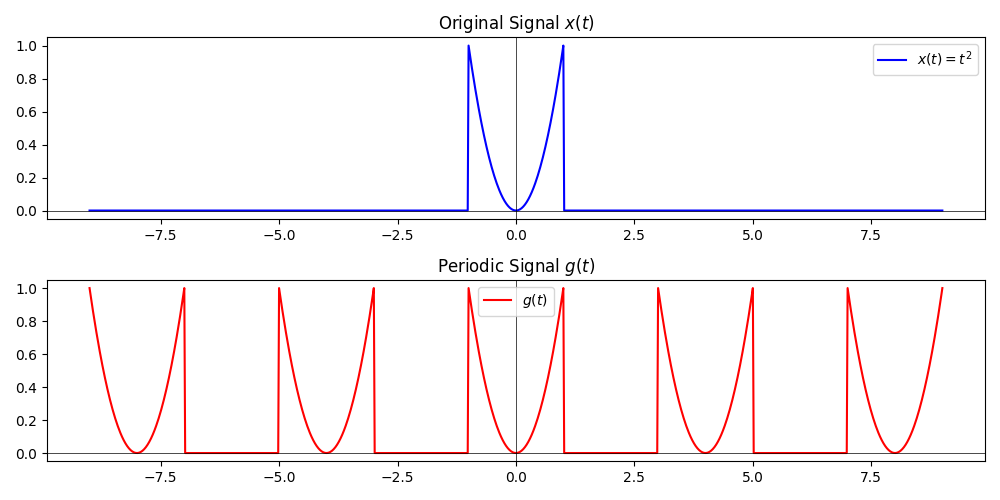
\includegraphics[width=0.75\textwidth]{p5.png}
        \caption{Plot of $x(t)$ and $g(t)$, The selected parameters are $T = 4$ and $\tau = 2$}
        \label{fig:p5}
    \end{figure}

    \item The fourier series coefficients of $g(t)$ are:
    \begin{align*}
        g_n &= \frac{1}{T} \int_{-T/2}^{T/2} g(t) e^{-j2\pi n t/T} dt \\
        &= \frac{1}{T} \int_{-T/2}^{T/2} \sum_{k=-\infty}^{\infty} x(t - kT) e^{-j2\pi n t/T} dt \\
        &= \frac{1}{T}\sum_{k=-\infty}^{\infty} \int_{-\tau/2}^{\tau/2} x(t - kT) e^{-j2\pi n t/T} dt, \quad \text{Let } u = t - kT \\
        &\text{The bounds can be set to } -\tau/2, \tau/2 \text{ as } x(t) \text{ is } 0 \text{ outside of this range} \\
        &= \frac{1}{T}\sum_{k=-\infty}^{\infty} \int_{\tau/2}^{-\tau/2} x(u) e^{-j2\pi n (u + kT)/T} du \\
        &= \frac{1}{T}\sum_{k=-\infty}^{\infty} e^{-j2\pi n k} \int_{\tau/2}^{-\tau/2} x(u) e^{-j2\pi n u/T} du \\
        &\text{We know that for any integer } n, k, e^{-j2\pi nk} = 1 \\
        &= \frac{1}{T}\int_{\tau/2}^{-\tau/2} x(u) e^{-j2\pi \left(\frac{n}{T}\right)u} du \\
        &= \frac{1}{T} X\left(\frac{n}{T}\right)
    \end{align*}
\end{enumerate}

\section{Problem 6}

\begin{enumerate}[label=6.\arabic*]
    \item Since $h(t)$ is an odd function, the fourier transform will be purely imaginary, and will have a phase of $\pm \frac{\pi}{2}$.
    \item Evaluating the following integral:
    \begin{align*}
        \int_{-\infty}^{\infty} G(f)\cos(\pi f)df &= \int_{-\infty}^{\infty} G(f)\left(\frac{e^{j\pi f} + e^{-j\pi f}}{2}\right)df \\
        &= \frac{1}{2}\int_{-\infty}^{\infty} G(f)e^{j\pi f}df + \frac{1}{2}\int_{-\infty}^{\infty} G(f)e^{-j\pi f}df \\
        &= \frac{1}{2}\int_{-\infty}^{\infty} G(f)e^{j2\pi f (\frac{1}{2})}df + \frac{1}{2}\int_{-\infty}^{\infty} G(f)e^{j2\pi f (-\frac{1}{2})}df \\
        &=\frac{1}{2}\left( g\left(\frac{1}{2}\right) + g\left(-\frac{1}{2}\right) \right) \\
        &= \frac{1}{4}
    \end{align*}
    \item Evaluating the following integral:
    \begin{align*}
        \int_{-\infty}^{\infty} H(f)e^{j4\pi f} df &= \int_{-\infty}^{\infty} H(f)e^{j2\pi f (2)} df \\
        &= h(2) \\
        &= 0
    \end{align*}

    \item The plot of the odd and even parts of $g(x)$ are shown in \autoref{fig:p6}.

    \begin{figure}[ht!]
        \centering
        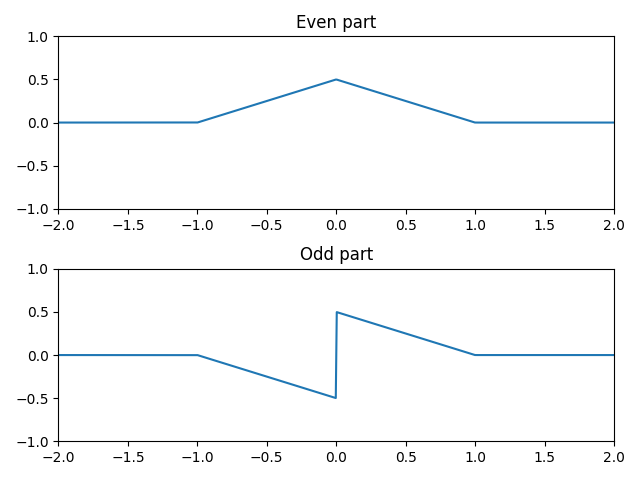
\includegraphics[width=0.5\textwidth]{p6.png}
        \caption{Plot of the odd and even parts of $g(x)$}
        \label{fig:p6}
    \end{figure}

    \item The real part of $G(f)$ is fourier transform of the even part of $g(t)$:
    \begin{align*}
        G(f) &= \int_{-\infty}^{\infty} g(t)e^{-j2\pi ft} dt \\
        &= \int_{-\infty}^{\infty} (g_e(t) + g_o(t))e^{-j2\pi ft} dt \\
        &= \int_{-\infty}^{\infty} g_e(t)e^{-j2\pi ft} dt + \int_{-\infty}^{\infty} g_o(t)e^{-j2\pi ft} dt \\
        &= \int_{-\infty}^{\infty} g_e(t) cos(2\pi ft) dt + j\int_{-\infty}^{\infty} g_o(t)sin(2\pi ft) dt \\
        &= \mathcal{F}\{g_e(t)\} + j\mathcal{F}\{g_o(t)\}
    \end{align*}

    In \autoref{fig:p6} we see that the even part of $g(t)$ is a triangle function, which has a fourier transform of a sinc$^2$ function. Which is:
    \begin{align*}
        g_e(t) = \frac{1}{2} \Lambda(t) \implies \text{Re}(G(f)) = \frac{1}{2} \text{sinc}^2(f)
    \end{align*}

    \item We can find the fourier transform of $g(t)$ as follows:
    \begin{align*}
        G(f) = \int_{-\infty}^{\infty} g(t)e^{-j2\pi ft}dt &= \int_{0}^{1}(1-t)e^{-j2\pi ft}dt \\
        &= \int_{0}^{1} e^{-j2\pi ft}dt - \int_{0}^{1} te^{-j2\pi ft}dt \\
        &= \frac{e^{-j2\pi f t}}{-j 2\pi f} \Bigg|_{0}^{1} - \left(\frac{te^{-j2\pi f t}}{-j2\pi f} \Bigg|_{0}^{1} - \int_{0}^{1} \frac{e^{-j2\pi f t}}{-j2\pi f}dt\right) \\
        &= \frac{1-e^{-j2\pi f}}{j2\pi f} - \left(\frac{e^{-j2\pi f}}{-j2\pi f}
        - \left(\frac{e^{-j2\pi f t}}{(-j2\pi f)^2}\right) \Bigg|_{0}^{1}\right) \\
        &= \frac{1}{j2\pi f} - \frac{e^{-j2\pi f}}{j2\pi f} + \frac{e^{-j2\pi f}}{j2\pi f} + \frac{e^{-j2\pi f} - 1}{(-j2\pi f)^2} \\
        &= \frac{-j}{2\pi f} + \frac{1-\cos(2\pi f) + j \sin (2\pi f)}{(2\pi f)^2} \\
    \text{Using the idenity: } 1-\cos(2x) &= 2\sin^2(x) \\
        &= \frac{-j}{2\pi f} + \frac{2\sin^2(\pi f) + j\sin(2\pi f)}{(2\pi f)^2} \\
        &= \frac{2\sin^2(\pi f)}{4(\pi f)^2}+ j\left(\frac{\sin(2\pi f)}{(2\pi f)^2} - \frac{1}{2\pi f}\right) \\
        &= \frac{\text{sinc}(f)^2}{2} + j\left(\frac{\text{sinc}(2f)}{2\pi f} - \frac{1}{2\pi f}\right) \\
        &= \boxed{\frac{\text{sinc}(f)^2}{2} + j\left(\frac{\text{sinc}(2f) - 1}{2\pi f}\right)}
    \end{align*}

    \item We can see that $h(t) = 2g_o(t)$, and thus the fourier transform of $h(t)$ is:
    \begin{align*}
        H(f) = j2\text{Im}(G(f)) = j \frac{\text{sinc}(2f) - 1}{\pi f}
    \end{align*}

    \item Given that $\varphi(x)$ is the periodized version of $h(x)$ with period $T=2$, we can use the result in \textbf{5.3} to find the fourier series coefficients $\varphi_n$:
    \begin{align*}
        \varphi_n = \frac{1}{T} H\left(\frac{n}{T}\right) = \frac{1}{2} H\left(\frac{n}{2}\right) &= \frac{j}{2} \frac{\text{sinc}(n) - 1}{\pi \frac{n}{2}} \\
        &= j\left(\frac{\text{sinc}(n) - 1}{n\pi}\right)
    \end{align*}
\end{enumerate}

% --------------------------------------------------------------------------------
% END BODY
% --------------------------------------------------------------------------------

\end{document}
ßf